\documentclass[12pt,a4paper,hidelinks]{article}
\input{premable}
\textwidth=450pt\oddsidemargin=0pt
\numberwithin{equation}{section}
\begin{document}

\begin{titlepage}
\begin{center}
\begin{spacing}{1.5}
\includegraphics[]{figures/frontespizio.png}\\
{{\Large{\textsc{DIPARTIMENTO DI INGEGNERIA DELL'INFORMAZIONE}}}}\\
{\large{\it Corso di Laurea in Ingegneria Informatica}}
\end{spacing}
\end{center}
\vspace{15mm}
\begin{center}
\begin{spacing}{1.5}

{\large Tesi di Laurea}

{\LARGE{\textsc{Tour scheduling e shift assignment: il caso di un supermercato}}}\\
% Concorde will fly
\end{spacing}
\end{center}
\vspace{35mm}
\par
\noindent
\begin{minipage}[t]{0.7\textwidth}

{\large{\bf Relatrice:\\ }}
\end{minipage}
\hfill
\begin{minipage}[t]{0.3\textwidth}
{\large{\bf Laureando:\\
Lublanis Matteo}}
\end{minipage}
\begin{minipage}[t]{0.7\textwidth}
\hfill
\end{minipage}
\hfill
\begin{minipage}[t]{0.3\textwidth}
{\large{\bf Matricola n.\\
736418}}
\end{minipage}

\vspace{25mm}
\begin{center}
{\large{\it Anno Accademico 2024/2025 }}
\end{center}
\end{titlepage}

\tableofcontents

% inserisci i file contenenti le sezioni

\section*{Introduzione}
\addcontentsline{toc}{section}{Introduzione}
\subsection{Personnel Scheduling: definizione e caratteristiche}
Un problema di Personnel Scheduling consiste nel trovare il modo migliore per attribuire i turni ai lavoratori, in modo tale sia da rispettare una serie di vincoli di servizio e contrattuali e sia da massimizzare le preferenze del personale riducendo comunque al minimo i costi previsti \cite{RENATOBRUNIPERSONNELSCHEDULING}.

Negli ultimi decenni, i problemi di schedulazione del personale sono stati studiati ampiamente. Una delle cause principali dietro questo interesse sta il lato economico: il costo del lavoro rappresenta ad oggi, per molte realtà aziendali, uno degli elementi principali della spesa aziendale e riuscire a minimizzarlo può portare grossi benefici all'azienda.\\
La prima formulazione di questo problema venne proposta negli anni '50 da George Dantzig e William Edie, ma ad oggi risulta antiquata in quanto:
\begin{itemize}
	\item Non esistevano diverse tipologie di contratto, solo contratti full-time.
	\item Ogni dipendente è interscambiabile, non vengono tenute in considerazione le skill del singolo individuo.
	\item Come obiettivo vi era solo quello di minimizzare il costo del personale, non considerando altri fattori come preferenze o indisposizioni. 
\end{itemize}
Baker fornì una classificazione dei problemi di Personnel Scheduling in tre gruppi\cite{VANDENBERGH2013367}:
\begin{itemize}
	\item Shift Scheduling: si pianifica su un orizzonte di pianificazione giornaliero, implicando che il fabbisogno di personale per ciascun turno può essere gestito in modo indipendente per determinare le allocazioni appropriate; rappresenta il problema più facile da risolvere delle tre categorie, ma non risponde a situazioni più complesse (esempio, la necessità dei turni che si sovrappongono, tipico problema per i call center).
	\item Days off Scheduling: al posto di pianificare i turni di lavoro, si pianificano i giorni di riposo per i dipendenti; problema tipico per aziende che lavorano sette giorni su sette, mentre il lavoratore ne lavora solo cinque/sei (una variante del problema potrebbe richiedere che i giorni di riposo siano consecutivi).
	\item Tour scheduling: una combinazione delle due categorie viste precedentemente, bisogna assegnare un tour (giorni della settimana e ore del giorno) da lavorare ad un particolare dipendente. Questa categoria risulta molto più complicata rispetto alle due precedenti e la complessità del problema, seppur dipenda da più fattori, è fortemente influenzata dalla durata minima dell'intervallo di pianificazione (solitamente, dai 15 minuti alle 8 ore).
\end{itemize}
Altre pubblicazioni suddividono il problema in moduli che poi possono essere uniti (demand modeling, days off scheduling, shift scheduling, $\cdot$), altre ancora danno una tassonomia del problema più dettagliata basata sulle seguenti caratteristiche:
\begin{itemize}
	\item Caratteristiche del personale;
	\item Vincoli, misure della performance e flessibilità;
	\item Metodi risolutivi e incorporazione dell'incertezza;
	\item Area applicativa e applicatività della ricerca.
\end{itemize}
In Ricerca Operativa, il Personnel Scheduling è un problema di tipo NP-hard, o peggio NP-complete: la complessità deriva principalmente da tutte le possibili combinazioni dei turni che si possono ottenere, rendendo la ricerca di un ottimo molto più complessa e lunga. Per modellizare il problema, può essere d'aiuto la definizione del problema di Set Covering, che riesce a modellizzare in maniera adeguata come l'unione dei turni assegnati debba rispondere al fabbisogno necessario. Nel problema di Set Covering bisogna trovare la più piccola sotto-collezione di set tale per cui l'unione dei suoi elementi sia equivalente all'insieme universo:
\begin{align*}
	\min \quad & \sum_{s\in S}x_s \\
	\text{s.t} & \sum_{s:e\in s}x_s\ge 1, \forall e\in U\\
	& x_s \in \{0, 1\}
\end{align*}
Nel caso del Personnel Scheduling, i sottoinsiemi rappresentano i turni e gli elementi gli slot temporali, il secondo vincolo cambierà in:
\begin{center}
	$\sum_{s:e\in s}x_s\ge f, \forall e\in U$
\end{center}
ove $f$ rappresenta il fabbisogno necessario per slot temporale.

Il problema è in continua evoluzione e necessita quindi modelli complessi e flessibili a eventuali cambiamenti. Gli strumenti risolutivi oggi disponibili (Gurobi, CPLEX, FICO Xpress, Google OR-Tools) integrano algoritmi sempre più raffinati: un problema che decenni fa veniva approcciato manualmente ottenendo risultati approssimativi, può ora essere risolto con precisione, garantendo soluzioni di alta qualità o, in molti casi, l’ottimalità globale.\\

\subsection{Obiettivo e struttura della tesi}
Questa tesi si pone come obiettivo quello di risolvere il problema di personnel scheduling (tour scheduling) per il reparto di cassa di un supermercato. Il fine ultimo è quello di trovare la miglior pianificazione settimanale possibile per suddetto supermercato e sviluppare uno strumento applicativo software per permettere un'assegnazione dei turni semplificata ai dipendenti.

Nel Capitolo 1 viene presentato informalmente il problema reale considerato, descrivendone i soggetti coinvolti, le preferenze espresse, ciò che si vuole ottenere e i vincoli di varia natura.

Nel Capitolo 2 viene delineato lo stato dell'arte nel settore, andando a individuare una definizione tecnica precisa per il tipo di problema individuato e andando a descrivere altre eventuali applicazioni degli stessi concetti che andremo a trattare nel corso della tesi.

Nel Capitolo 3 si fornisce la descrizione formale del problema, che verrà tradotta in un vero e proprio modello matematico, riportato all'interno del Capitolo 4.

Nel Capitolo 5 illustra lo strumento utilizzato per l’implementazione del modello matematico (Gurobi), le principali fasi del processo di realizzazione e i risultati dei test sperimentali volti a valutarne l’efficienza e la validità. 

Nel Capitolo 6, una volta terminata la formulazione del piano orario, si definisce il meccanismo di assegnamento dei turni.

Negli appendici infine vengono riportati, per ordine:
\begin{itemize}
	\item Una guida sintetica per l'utilizzo del programma finale, accompagnata da alcuni frammenti di codice commentati.
	\item Valori dei coefficienti di penalità assegnati ai termini della funzione obiettivo.
\end{itemize}

\section{Descrizione del problema}

\subsection{Introduzione}
La formulazione di un piano orario per i propri dipendenti risulta fattibile fin quando la dimensione del personale da gestire rimane contenuta e fin quando non si tengono in considerazione variabili secondarie come preferenze del personale e limiti giuridici.
 
Consideriamo il problema di turnazione per un roster di cassieri di un ipermercato, appartenente alla grande distribuzione organizzata, affermatosi nella realtà bresciana. Il piano di turnazione viene stilato settimanalmente dal caporeparto delle casse e può richiedere fino a due/tre giorni di lavoro intenso, spesso non riuscendo a trovare una soluzione adeguata al flusso della clientela e alle esigenze del punto vendita, creando inoltre disagio all'interno del personale. 

Si richiede, quindi, di formulare una piano di turnazione standard e poi di risolvere il problema di assegnamento dei dipendenti ai corrispettivi turni, sia rispettando i vincoli contrattuali e sia andando incontro a esigenze di varia natura (aziendali e dei singoli dipendenti), in modo tale da non solo ottimizzare i tempi lavorativi necessari alla pianificazione settimanale ma anche riuscire a ridurre i costi e a massimizzare la soddisfazione del personale.\\ 

\subsection{Settimana lavorativa}
L'ipermercato opera 7 giorni su 7, con un orario continuato per la clientela dalle 08:00 fino alle 20:00. Tralasciando le festività nazionali (Natale, Ferragosto, Festa dei lavoratori, $\dots$), è aperto tutto l'anno.

L'orario per un cassiere normale va dalle 08:00 fino alle 20:30, mezz'ora dopo la chiusura dell'ipermercato, in modo tale da poter eseguire le attività finali necessarie, come conteggio dei contanti e pulizie. Alle 07:00 è richiesta invece l'utilizzo della spazzatrice per poter pulire le corsie: solo alcuni dipendenti possiedono la formazione necessaria per poter adoperare la spazzatrice, dipendenti ai quali sarà richiesto di iniziare il turno prima rispetto agli altri.

\subsection{Tipologia personale, caratteristiche turnazione}
Il personale è suddiviso in tre categorie contrattuali:
\begin{itemize}
	\item Full time: 40 ore settimanali;
	\item Part time: 24    settimanali;
	\item Part time weekend: 20 ore settimanali, con disponibilità limitata ai giorni di venerdì, sabato e domenica.
\end{itemize}
Ogni singolo turno può durare dalle 3 alle 6 ore. Non sono previste pause in un turno, ma sono previsti due turni giornalieri per i lavoratori full-time e part-time fine settimana (solo il sabato e la domenica per loro); quindi, ci sarà uno stacco tra due turni giornalieri, che può variare da una mezz'ora fino a quattro ore e mezza.
Un dipendente può lavorare fino a 12 ore al giorno, ma è una situazione indesiderata: si tende ad assegnare fino ad un massimo di 8 ore al giorno ad ogni singolo dipendente, con piccole variazioni di mezz'ora in positivo o in negativo in base alle esigenze. Ad un dipendente si possono assegnare fino ad un massimo di 48 ore settimanali (ore previste da contratto più straordinari), ma si vuole rimanere il più possibile vicini ai monte ore previsti da contratto: questo vale anche per i part-time, i quali prima delle 40 ore lavorerebbero ore supplementari e non straordinarie.

Tra l'ultimo turno del giorno precedente e il primo turno del giorno preso in considerazione, vi deve essere un riposo di almeno 11 ore previsto per legge. Considerando la struttura degli orari (senza considerare chi deve passare la spazzatrice), si rispetta tranquillamente il vincolo, però risulta comunque preferibile una pausa tra due turni in giorni consecutivi la più lunga possibile, così da permettere un riposo maggiore al dipendente.

\subsection{Richieste del caporeparto}
Il caporeparto è il soggetto che predispone il fabbisogno per ogni singolo slot temporale, in modo tale da poter pianificare il personale rispondendo in maniera adeguata al flusso della clientela e alle esigenze del punto vendita. Il caporeparto fornisce una tabella settimanale, di cui ogni singola cella rappresentano il numero di dipendenti richiesto per un certo slot orario: ad esempio, il sabato, essendo il giorno più intenso per l'ipermercato, avrà un fabbisogno molto più elevato rispetto ad un giorno infrasettimanale come il martedì.

Il fabbisogno è un numero indicativo di quante persone siano necessarie in quel momento; non è un limite obbligatorio, quindi possono esserci situazioni di sotto o sovra copertura. La situazione di sovracopertura è preferibile rispetto a quella di sottocopertura solo nel caso in cui vi siano dipendenti che possano andare in scatolame durante situazioni di basso flusso della clientela: una situazione di eccesso di personale in cassa non solo risulterebbe inutile, ma verrebbe anche malvisto dai clienti, che vedrebbero dei dipendenti fermi.

Il caporeparto vuole riuscire a coprire il fabbisogno richiesto, limitando il più possibile il monte ore lavorato totale, così da limitare le spese del personale. 

Infine, il caporeparto vuole assicurarsi di riuscire a rispondere a situazioni critiche, in quanto il disagio arrecato da imprevisti potrebbe danneggiare l'immagine dell'ipermercato.

\subsection{Skill del personale}
Skill particolari individuate durante la descrizione del problema sono:
\begin{itemize}
	\item Cassa-Reparto: alcuni cassieri possono essere assegnati sia nel reparto scatolame che alle casse, differenziandoli così dai puri cassieri, che una volta assegnati allo slot temporale dovranno per forza stare in cassa. 
	\item Formazione spazzatrice: alcuni dipendenti possiedono la formazione necessaria per adoperare la spazzatrice; tali dipendenti possono iniziare a lavorare prima delle 08:00 per poter così pulire l'ipermercato entro l'apertura.
\end{itemize}

\subsection{Preferenze del personale}
Oltre ai vincoli contrattuali, si vuole tenere conto di alcune preferenze espresse dai dipendenti, che contribuiscono a migliorare la soddisfazione e l’equità complessiva della pianificazione.\\
In particolare, vengono considerate le seguenti preferenze:
\begin{itemize}
	\item che vi sia equità nella distribuzione del carico lavorativo;
	\item avere giorni di riposo consecutivi;
	\item ridurre al minimo gli stacchi tra due turni nello stesso giorno (favorendo turni continuativi);
	\item disporre del riposo domenicale, ove possibile.
\end{itemize}

\subsection{Obiettivi finali}
La formulazione del piano dei turni mira al raggiungimento di più obiettivi:
\begin{itemize}
	\item Minimizzare i costi del personale;
	\item Massimizzare la soddisfazione del personale;
	\item Mantenere flessibilità operativa, in modo da poter gestire eventuali imprevisti (assenze, malattie, permessi, variazioni della domanda).
\end{itemize}
In sintesi, il problema affrontato è un problema di ottimizzazione combinatoria tipico del rostering/staff scheduling.

Richiede di assegnare, per un periodo prefissato (una o due settimane, un mese o addirittura un anno), un insieme di turni ai lavoratori disponibili, in modo da soddisfare i vincoli di copertura, orario e riposo, cercando contemporaneamente di ottimizzare più criteri di tipo economico e organizzativo.


\section{Stato dell'arte}
Nel 2012, l'European Journal of Operational Research pubblicò un articolo chiamato \textit{Personnel scheduling: A literature review}\cite{VANDENBERGH2013367}, nel quale un team di sei ricercatori ha raccolto 291 articoli per dare un quadro generale sullo stato dell'arte dal 2004 fino ad allora, definendone anche una tassonomia. Questo capitolo si concentrerà su questa pubblicazione, andando nel dettaglio per alcuni documenti citati e aggiungendo documenti più recenti. La tassonomia per i problemi di Personnel Scheduling si basa su quattro campi: caratteristiche del personale, vincoli assieme a misure di performance e flessibilità, metodi risolutivi e incorporazione dell'incertezza, area applicativa e applicabilità della ricerca.
\subsection{Caratteristiche del personale}
La prima caratteristica del personale che si definisce è la tipologia di contratto: la maggior parte delle pubblicazioni scientifiche riguardante questo problema trattanto problemi in cui il personale è per intero di tipo full-time. L'articolo di Hojati e Patil \cite{HOJATI201137} è uno dei pochi che va a trattare la categoria dei contratti part-time per intero. Nel caso dei contratti part-time, la gestione dei turni diventa molto più articolata, in quanto bisogna tenere in considerazione nuovi problemi, come la disponibilità dei dipendenti rispetti a giorni specifici o anche la richiesta necessaria per l'azienda. 

In alcuni problemi, le attività possono richiedere alcune skill specifiche, rendendo così il personale considerato ancora più eterogeneo rispetto alla suddivisione "full-time/part-time"; si considerano anche i casi in cui tali attività possono essere svolte da persone che non possiedono le skill necessarie, comportando però un aumento del costo, in quanto saranno ovviamente meno efficienti rispetto al personale qualificato. Le skill specifiche sono in stretto legame con i livelli di produttivitià e anzianità: allo stesso modo della classificazione in base alle skill, un lavoratore meno produttivo equivarrà ad un costo aumentato. Sia la produttività che l'anzianità possono essere combinate assieme, anche con altre skill. In particolare, per l'anzianità possono essere previsti dei privilegi, come giorni di riposo consecutivi o un peso maggiore che viene dato alle loro preferenze per gli orari.

Un'altra classificazione si basa sul raggruppamento degli impiegati: questo è molto utile in problemi dove si considera lo scheduling di un team di persone e non ogni dipendente individualmente, come ad esempio problemi legati all'area dei trasporti, dove si lega il problema di Personnel Scheduling con quello del routing di veicoli. Esempi per questo tipo di problemi sono l'articolo di Sydney C.K. Chu\cite{CHU20071764} o anche l'articolo di Heil, Hoffmann e Buscher\cite{HEIL2020405}, che si preoccupa di inquadrare nel dettaglio i problemi di crew scheduling per il trasporto ferroviario.
%shine on you crazy diamond
Nell'articolo viene anche definita una tassonomia sulla base del tipo di decisioni che devono essere prese (assegnamento delle attività, sequenza dei turni, tempo, altro) e vengono separati in base a se vengono prese per interi team o per singoli membri del personale. Un esempio che evidenzia la tassonomia basata sulle decisioni si ritrova nell'articolo di Horn et al.\cite{Horn01102007}, che si occupa di trovare il modo più efficiente per la Forza di pattugliamento della Royal Australian Navy di utilizzare una nuova generazione di barche militari. Osservando la letteratura, si può notare che la maggior parte degli articoli si occupa solamente di creare una turnazione accettabile o una schedulazione dei lavori per i dipendenti, dato un carico di lavoro deterministico. Quasi mai, questo problema viene integrato con altri problemi di pianificazione, come la pianificazione del personale, previsione e adeguamento della distribuzione del carico di lavoro, distribuzione delle pause, assunzione e licenziamento, formazione,$\dots$. Diventa importante questo per la ricerca futura: cercare di unire tutte le decisioni in un unico problema di scheduling.

Anche la flessibilità con il tempo ha assunto un ruolo fondamentale, rendendo ancora di più complicata la formulazione dei modelli per i problemi considerati. La flessibilità può riguardare: sovrapponibilità dei turni, diversi orari di inizio, diverse lunghezze dei turni, diverse durate delle pause, $\dots$. 

Le scelte decisionali prese per lo scheduling diventano fondamentali non solo per questioni economiche, ma anche per la questione psicologica e fisica dei lavoratori. Xu e Hall\cite{XU2021807} pubblicarono un articolo riguardante la fatica lavorativa, introducendola come variabile all'interno dei problemi di scheduling: un lavoratore stanco rende di meno, aumentando di conseguenza il costo complessivo. L'articolo va ad analizzare quanto in letteratura venga misurata e analizzata la fatica e quale sia il suo impatto sulla performance, andando ad analizzare l'impatto che scelte di scheduling possono avere su di essa. Questo tema si lega strettamente al concetto di flessibilità, in quanto uno schema rigido non può rispondere ad una situazione variabile come la fatica di un lavoratore e bisognerà introdurre nuovi concetti, come quello delle rate-modifying activity (RMA, azioni che cambiano la velocità di produzione di una macchina) o delle micro-pause.

\subsection{Vincoli e Obiettivi}
Si differenziano i vincoli in hard e soft, ove con hard si indicano vincoli che non possono essere violati, mentre soft sono vincoli più flessibili. Nell'articolo vengono definite le seguenti categorie per i vincoli: copertura, temporali, equità e di equilibrio.

I vincoli di copertura rappresentano un aspetto chiave per i problemi di personnel scheduling: sia i vincoli hard che i vincoli soft di copertura stanno alla base dell'intero problema di scheduling, ovvero la scelta del numero di dipendenti necessari per coprire un carico di lavoro. I vincoli di copertura vanno contro solitamente la funzione obiettivo, che cerca di minimizzare la forza lavoro totale, in quanto direttamente legata al costo. La differenza tra capacità del personale minima e ottima è di fondamentale interesse per chi si occupa di questi problemi, in quanto rende necessario affrontare problemi come l'eccesso o il difetto di personale. All'interno dell'articolo, vengono riportati alcuni documenti che vanno anche a trattare problemi che vanno al di là della semplice gestione dei turni del personale, come la carenza di personale a livello internazionale per problemi di scheduling di infermieri: una possibile soluzione è quella di definire i vincoli di copertura come soft, prevedendo l'introduzione di personale esterno per coprire buchi all'interno della pianificazione e tenendo come obiettivo quello di generare un insieme di roster che minimizzino il numero di turni scoperti durante il lasso temporale considerato. L'utilizzo di vincoli hard implica quasi sempre, all'interno della letteratura trovata, un divieto per l'understaffing: nell'articolo, viene citato un singolo caso in cui la situazione è invertita ed è dovuto a motivi finanziari (sempre legati alla mancanza di personale). Altra cosa che si potrebbe implementare nella copertura riguarda le pause, però essendo un problema di tipo principalmente real-time non vengono trattate all'interno delle pubblicazioni sui problemi di personnel scheduling (Thompson e Pullman han dedicato un intero articolo soltanto alla gestione delle pause\cite{THOMPSON2007139}, andando ad analizzarne i pro e i contro di una organizzazione delle pause anticipata).

Se il personale può essere caratterizzato da delle skill, si introducono solitamente vincoli hard per assicurarsi la presenza di dipendenti qualificati per lo svolgimento di un particolare lavoro. I vincoli soft in questo caso possono venire utilizzati per indicare una possibile introduzione di personale non adatto all'attività considerata, implicando però un aumento del costo, o anche possono rappresentare il concetto di skill alternative, ovvero dipendenti che possiedono diverse skill ma che preferiscono evitare di coprire certi tipi di lavoro. Si distinguono tre diversi gruppi in base al grado di flessibilità delle competenze:
\begin{itemize}
	\item Le skill sono definibili a livello di dipendente, ovvero chi pianifica ha piena libertà di scegliere le skill per ogni membro del personale.
	\item L'insieme dei dipendenti viene gerarchizzato: dipendenti a livelli superiori possono eseguire attività dei dipendenti a livelli inferiori, mentre non vale il contrario; fattori su cui si può basare la gerarchia sono esperienza, dipendenti junior/senior, background formativo, $\dots$
	\item Le skill non possono essere sostituite, alcune attività richiedono skill specifiche e possono essere svolte solo da lavoratori con quelle particolari skill.
\end{itemize}

Altro problema importante è quello degli straordinari, il cui utilizzo può influenzare molto sulla flessibilità della copertura. Gli straordinari possono essere limitati settimanalmente, oppure possono essere studiati su orizzonti temporali più ampli, lasciando più libertà di gestione degli orari settimanali: un esempio nel quale lo studio delle ore complessive viene fatto mensilmente è il caso studiato nella tesi di Serena Cortopassi\cite{etd-04172014-181428}, dove viene studiato un problema di personnel scheduling per il personale de Il Gignoro, una residenza assistenziale per anziani. 

Le misure finanziarie prevedono costi differenti, come costo del personale, possibile costo relativo ad un particolare giorno della settimana, diversi costi per diverse skill, costo degli straordinari, costo legato allo svolgimento di particolari attività, $\dots$: minimizzare il costo è strettamente legato al minimizzare il numero di dipendenti usati, ma questo non significa che è solo questo ma è anzi un problema molto più complesso che va analizzato. Già modellare il costo del problema attorno al costo del personale invece che il numero dei dipendenti, si riesce ad ottenere un compromesso tra assunzione di dipendenti, straordinari, lavoratori occasionali e altro. Altri possibili costi possono essere costi di produzione, costi per chiamate perse o mancata produzione, costi differenti tra lavoratori full-time e part-time, costi di rifiuto, costi differenti per sede, $\dots$.

Spesso gli operatori vogliono anche garantire equità nella gestione degli orari per i dipendenti, che si può tradurre in più punti: distribuzione equa di weekend di riposo, un numero di turni sfavorevole bilanciato tra i vari dipendenti, gestione bilanciata per tipo di turno, quantità bilanciata di giorni di lavoro e di riposo (viene citato il lavoro di Lezaun e altri\cite{lezaun2007rostering}), gestione delle preferenze dei dipendenti (ad esempio, preferenze per certi tipi di turni o anche volere lavorare con specifici collaboratori), numero di giorni di riposo consecutivi), $\dots$.

\subsection{Metodi Risolutivi e Incertezza}
In letteratura, si trova un insieme veramente ampio e diversificato di tecniche risolutive adottate. Si dividono le tecniche usate in tre gruppi:
\begin{itemize}
	\item Programmazione matematica: programmazione intera, programmazione dinamica, goal programming, euristiche costruttive o migliorative.
	\item Simulazione, programmazione a vincoli, queuing.
	\item Altro: soluzioni meno frequenti come approssimazione lineare a tratti di una curva, analytic hierarchy process (AHP), modelli di fogli di calcolo e data envelopment analysis (DEA).
\end{itemize}
Il primo gruppo rappresenta il gruppo più ampio: il problema del personnel scheduling viene modellato come un programma lineare, intero o misto intero e la formulazione più usata è quella del Set Covering, introdotta da Dantzig. Il problema del \textit{Set Covering} consiste nel trovare la più piccola sotto-collezione di insiemi (sottoinsiemi dell'insieme universo) tale per cui l'unione dei suoi elementi sia equivalente all'insieme universo:
\begin{align*}
	\min \quad & \sum_{s\in S}x_s \\
	\text{s.t} & \sum_{s:e\in s}x_s\ge 1, \forall e\in U\\
	& x_s \in \{0, 1\}
\end{align*}
In particolare, nel caso del personnel scheduling, al posto dell'1 nel secondo vincolo si avrà il fabbisogno necessario per lo slot temporale considerato. Questa formulazione è molto comoda, perché permette di aggiungere a proprio piacimento vincoli aggiuntivi in base alle proprie necessità. 

Una tecnica che aiuta molto, in particolare per problemi di larga scala, è quella della decomposizione del problema: viene separato il problema in due parti, una più facile e una più complessa e per ognuna posso scegliere il metodo risolutivo da utilizzare. Diversi modi di applicare la decomposizione furono proposti da: Detienne e altri\cite{detienne2009cut} sfruttarono la decomposizione di Bender (problema principale rilassato è un problema di zaino multidimensionale a multiscelta, mentre ogni sotto problema è un problema di b-matching\footnote{Generalizzazione del problema base di matching per un grafo. Sia dato un grafo $G=(V,E)$, ad ogni vertice $v\in V$ viene assegnato una capacità $b(v)\in \mathbb{N}^+$: un b-matching è un sottoinsieme di archi tale che, per ogni $v$, il numero di archi incidenti a $v$ non superi la sua capacità $b(v)$.}, Bard e Wan\cite{bard2008workforce} \cite{bard2006task}. Assieme alla decomposizione, un'altra tecnica buona per problemi di grandi dimensioni è quella della generazione di colonne: quando le variabili in gioco sono troppe, si rischia di eccedere il limite di memoria assegnato per il problema, quindi vengono generate dinamicamente quando necessario\cite{IBMColonne} (vengono citati per questo approccio Beliën e Demeulemeester\cite{belien2008branch}). Tramite la decomposizione, si riesce ad utilizzare a rappresentare il problema con altri modelli oltre a quello del set covering, come ad esempio problemi di maximum flow.

Ultimo approccio molto utilizzato all'interno della programmazione matematica è quello delle metaeuristiche, che sono progettate in modo tale da trovare soluzioni ammissibili buone in tempi relativamente brevi o accettabili dai limiti imposti. Gli svantaggi delle metaeuristiche sosta nel fatto che non possono in modo dimostrabile né produrre soluzioni ottime né ridurre lo spazio di ricerca delle soluzioni. Gli algoritmi preferiti sono la tabu search e gli algoritmi genetici all'uso di algoritmi di ricottura simulata. Altre alternative sono: scatter search, ricerca locale iterata, variable neighborhood search, particle swarm optimization, algoritmi memetici, reti neurali, $\dots$.

Trattando invece l'incertezza, si differenziano tre tipi di incertezze che si possono ritrovare all'interno di questi problemi:
\begin{itemize}
	\item Incertezza della richiesta: carico del lavoro imprevedibile.
	\item Incertezza dell'arrivo: pattern imprevedibile dell'arrivo carico di lavoro (fallimenti della macchina, arrivo di chiamate per i call center).
	\item Incertezza della capacità: deviazione tra forza lavoro pianificata e effettiva.
\end{itemize}
Si dividono inoltre gli approcci in due tipi:
\begin{itemize}
	\item Deterministico: viene ignorata ogni forma di incertezza.
	\item Stocastico: viene considerata l'incertezza (non per forza tutti i tipi visti prima).
\end{itemize}
L'approccio deterministico è quello dominante. Non incorporare l'incertezza all'interno del modello non equivale però a considerare il carico di lavoro costante in ogni momento: vengono fatte analisi del carico di lavoro osservando i dati storici e facendone una stima. Per andare contro la variabilità del carico di lavoro, negli approcci deterministici può risultare d'aiuto l'utilizzo di buffer di capacità in modo tale da rendere il roster del personale molto più robusto.

Cause di incertezza relative ai dipendenti possono essere: malattie dei dipendenti, ritardi negli arrivi, perdita di capacità per via di risorse fuori servizio. L'incertezza di arrivo è di principale interesse per i sistemi di call center, i quali spesso devono aggiungere anche l'incertezza di richiesta.

\subsection{Aree di Applicazione}

\subsection{AI}

\section{Definizione formale}
In questa sezione, si offre una descrizione formale del problema mediante l'utilizzo di un modello di Programmazione Lineare Mista Intera (MILP), che verrà poi inserito come input in Gurobi, un risolutore matematico. Un modello si struttura nel seguente modo:
\begin{align*}
	\max_{x\in \mathbb{Z}^n} \quad & c^Tx \\
	\text{s.t.} \quad & Ax \leq b, \\
	& x \geq 0
\end{align*}
ove $\max_{x\in \mathbb{Z}^n} c^Tx$ rappresenta la funzione obiettivo che deve essere massimizzata o minimizzata, mentre le altre due righe rappresentano i vincoli del modello. Questa sezione è suddivisa in tre parti:
\begin{enumerate}
	\item Problema base: viene definito formalmente il minimo necessario per avere un modello base funzionante, senza andare incontro a vincoli aggiuntivi come skill o preferenze del personale.
	\item Problema esteso: vengono aggiunti i vincoli mancanti al problema base, analizzando anche quali elementi potrebbero andare in conflitto con quelli precedenti.
	\item Possibili estensioni. 
\end{enumerate}
\subsection{Problema base}

\paragraph{Insieme dei cassieri}
Si indica con $w$ un cassiere generico appartenente al roster. I cassieri si differenziano tra loro principalmente per gli orari contrattuali assegnati, introduciamo gli insiemi:
\begin{center}
	$W=FT\cup PT \cup PTW$\\
	$FT=\{w_1,...w_n\}$, full-time\\
	$PT=\{w_1,...w_p\}$, part-time\\
	$PTW=\{w_1,...w_k\}$, part-time weekend\\
	$FT\cap PT = \O$\\
	$FT\cap PTW = \O$\\
	$PT\cap PTW = \O$
\end{center}
ove $W$ rappresenta l'insieme di tutti i cassieri. Per adesso, le uniche differenze che vi sono tra i diversi cassieri sostano solo nel monte orario: appartenere ad un insieme, equivale a condividere la stessa paga oraria (stesso inquadramento lavorativo e stessa tipologia di contratto, nessuna anzianità) e lo stesso minimo di ore da lavorare con tutti gli altri dipendenti appartenenti allo stesso sottoinsieme.

\paragraph{Copertura oraria e turni}
Durante una giornata, l'obiettivo del caporeparto è quello di coprire il flusso della clientela in maniera adeguata. Rifacendoci al problema del \textit{Set Covering} e all'articolo di Brucker\cite{BRUCKER2011467}, si definiscono:
\begin{center}
	$D=\{lun, \dots , dom\}=\{1,\dots ,7\}$ l'insieme dei giorni settimanali, che rappresenta la finestra temporale (da 0, lunedì alle 7, fino all'ultimo slot, domenica alle 20).\\
	$f_{d,k}$ il fabbisogno per lo slot $k$ del giorno $d$.\\
	$K_d$ l'insieme degli slot del giorno $d$.
\end{center}
Gli slot temporali possono avere durata variabile, dall'intera giornata lavorativa fino a soli 15 minuti: si è deciso di utilizzare uno slot temporale di mezz'ora. La giornata di lavoro inizia alle 08:00 e finisce alle 20:30 (verrà modificato non appena si introdurranno i vincoli per la spazzatrice), è quindi suddivisa in 25 slot temporali. L'orario è continuato ed è identico per tutti e sette i giorni della settimana, dunque vi sarà da definire un totale di 175 fabbisogni, ognuno per il singolo slot $k$ della giornata $d$.
I turni assegnati ai dipendenti saranno gli insiemi tipici del \textit{Set Covering}. Specifichiamo:
\begin{center}
	$S=\{s_1, \dots , s_l\}$ l'insieme dei turni $s$
\end{center}
I turni $s$ sono caratterizzati da:
\begin{itemize}\label{defturno}
	\item $day(s)$: il giorno $d$ del turno $s$.
	\item $start(s)$: lo slot di inizio del turno $s$.
	\item $L_s$: durata ($\in \{6,7,\dots, 12\}$, misurata in slot) del turno $s$.
	\item $A_{s,k}$: copertura dello slot $k$ dal turno $s$ (1 se coperto, 0 altrimenti).
\end{itemize}
Gli slot temporali dovranno essere coperti da almeno $f_{d,k}$ turni. Per definire se un cassiere lavora o meno un certo turno, usiamo una variabile decisionale:
\begin{center}
	$x_{w,s}\in \{0,1\}$
\end{center}
la quale varrà 1 nel caso in cui al cassiere $w$ sia assegnato il turno $s$, 0 altrimenti. Unendola alla matrice di copertura $A_{s,k}$ possiamo così dire se un cassiere $w$, prendendosi in carico il turno $s$, copra o meno lo slot $k$.

I cassieri si differenziano per il monte orario minimo in base alla tipologia di contratto:
\begin{center}
	$C_{w}\in \{20,24,48\}$
\end{center}
Una volta introdotto il necessario per l'orario e la copertura, si può iniziare a definire i vincoli relativi: 
\begin{align}
	& \sum_{w \in W}\sum_{s \in S : day(s)=d} A_{s,k} x_{w,s} 
	\ge f_{d,k} 
	&& \forall d, k \label{vincolo:copertura}\\
	& C_{w} \le \sum_{w \in W, s} 0.5*L_sx_{w,s} \le 48
	&& \text{monte ore} \label{vincolo:monteorept}
\end{align}
La copertura del fabbisogno si specifica mediante il primo vincolo. Questo vincolo assicura che almeno $f_{d,k}$ cassieri siano presenti nello slot temporale $k$ del giorno $d$. Con questo vincolo non è ammissibile una situazione di difetto di personale, ma è ammissibile un eccesso di personale. Si potrebbe ammettere una situazione di difetto modificando il valore di $f_{d,k}$ o cambiando il peso del vincolo (introducendo ad esempio una nuova variabile $p_f$, il cui valore può ridurre o aumentare $f_{d,k}$).

Ogni cassiere deve lavorare almeno il monte orario minimo definito da contratto, ma può raggiungere le 48 ore facendo straordinari.

Gli ultimi vincoli riguardano il numero di turni giornalieri, che si ricorda sono:
\begin{displayquote}
	\textit{Part time weekend: 20 ore settimanali, con disponibilità limitata ai giorni di venerdì, sabato e domenica.\dots\\
	\dots ma sono previsti due turni giornalieri per i cassieri full-time e part-time fine settimana (solo il sabato e la domenica per loro)\dots Ai cassieri part-time viene assegnato un solo turno giornaliero.\\
	Un dipendente può lavorare fino a 12 ore al giorno, ma è una situazione indesiderata: si tende ad assegnare fino ad un massimo di 8 ore al giorno ad ogni singolo dipendente\dots}
\end{displayquote}
Si definiscono i seguenti vincoli:
\begin{align}
	& \sum_{w \in FT, \, s : day(s)=d} x_{w,s} \le 2, 
	&& \forall d \label{vincolo:ft}\\
	& \sum_{w \in PT, \, s : day(s)=d} x_{w,s} \le 1, 
	&& \forall d \label{vincolo:pt}\\
	& x_{w\in PTW,s} = 1, 
	&& day(s)=5 \land start(s)=16{:}30 \label{vincolo:weekend}\\[6pt]
	& x_{w\in PTW,s} = 0, 
	&& day(s)<5 \label{vincolo:weekend2}\\
	& \sum_{w \in PTW, \, s : day(s)=d} x_{w,s} \le 2, 
	&& d>5\label{vincolo:weekend3}
\end{align}
I primi due vincoli rappresentano i vincoli per i cassieri full-time e part-time, mentre gli ultimi tre sono i vincoli per i part-time fine settimana. Per richiesta del caporeparto, i cassieri part-time fine settimana il venerdì lavorano solo il turno della chiusura (dalle 16:30 alle 20:30), mentre il sabato e la domenica vengono trattati come cassieri full-time.

Si può infine introdurre la funzione obiettivo per questa parte:
\begin{equation}
	f_1=\sum_{w \in W}\sum_{s \in S} 0.5 L_s x_{w,s} 
\end{equation}
ovvero la somma totale delle ore lavorate dall'intero roster dei cassieri, che andrà minimizzata come da richiesta.

\paragraph{Stacco turni}
I cassieri hanno richiesto uno stacco tra due turni giornalieri il più breve possibile. Questo permetterebbe di ridurre al minimo il tempo trascorso sul luogo di lavoro e aumentare la soddisfazione del personale. Il problema si pone solo nel caso in cui il cassiere faccia due turni in un giorno:
\begin{align}
	& split_{w,d} \ge \sum_{s : day(s)=d} x_{w,s} - 1\\
	& split_{w,d} \in \{0,1\}
\end{align}
è una variabile decisionale, che ci dice se il cassiere $w$ è assegnato a due turni $s_1$ e $s_2$ nello stesso giorno $d$.

I turni $s$, per come sono \hyperref[defturno]{definiti}, permettono il calcolo dello slot di fine turno:
\begin{equation}
	end(s)=start(s)+L(s)
\end{equation}
e da questo si può trovare il valore dello stacco:
\begin{equation}
	stacco_{w,d} \ge  split_{w,d} \cdot (start(s_2) - end(s_1)), \quad \forall w \in W
\end{equation}
che viene considerato solo nel caso in cui effettivamente il cassiere abbia due turni lo stesso giorno. Devono valere di conseguenza anche:
\begin{align*}
	& x_{w,s_1} = x_{w,s_2} = 1,\\
	& day(s_1) = day(s_2),\\
	& start(s_2) > end(s_1). 
\end{align*}
Bisogna infine minimizzare:
\begin{equation}
	f_2=\sum_{d \in D}\sum_{w \in W} stacco_{w,d}
\end{equation}
ovvero gli stacchi di tutti i cassieri.

\paragraph{Giorni di riposo}
Si considera giorno di riposo un qualsiasi giorno della settimana nel quale il cassiere non è stato assegnato a nessun turno:
\begin{equation}
	r_{w,d} \ge 1-\sum_{s\in S_d}x_{w,s}, \quad \forall w\in W \setminus PTW,\forall d\in D
\end{equation}
Durante la settimana, il cassiere deve avere almeno un giorno di riposo e per evitare un sovraccarico di ore giornaliere può arrivare ad un massimo di due giorni di riposo settimanali:
\begin{equation}
	1 \le \sum_{d\in D} r_{w,d}\le 2
\end{equation}
Per i part-time fine settimana il problema non si pone, in quanto durante la settimana non gli si può assegnare turni.

\subsection{Problema esteso}
\paragraph{Straordinari}
Gli straordinari vengono penalizzati in quanto prevedono una retribuzione maggiorata, aumentando notevolemente il costo finale per il punto vendita. Si introduce:
\begin{center}
	$O_w\in \mathbb{N}$
\end{center}
che rappresenta le ore straordinarie assegnate al cassiere $w$. Questo valore è maggiore o uguale a 0 e si preferirebbe che valesse 0 per tutti i cassieri del roster. Non vale 0 nel caso in cui:
\begin{align}
	& O_w \ge \sum_{s \in S : day(s)=d} A_{s,k} x_{w,s} - C_{w} 
	&& \forall w \in W \label{vincolo:straordinari}
\end{align}
ovvero quando al cassiere $w$ vengono assegnate più ore di quelle previste dal contratto. La somma di questi valori va minimizzata:
\begin{equation}
	f_3=\sum_{w \in W}O_w
\end{equation}
Non si fanno distinzioni tra supplementari e straordinari: sono entrambi penalizzati allo stesso modo. Il peso assegnato a questo obiettivo può variare in base al periodo, rendendo più favorevoli gli straordinari in periodi più critici, come quelli festivi.

\paragraph{Equità}
I problemi riguardanti l'equità sono:
\begin{itemize}
	\item Carico orario settimanale uguale per tutti i cassieri dello stesso tipo.
	\item Carico orario giornaliero uguale per tutti i cassieri dello stesso tipo, ad esempio scatta una situazione di inequità nel momento in cui un cassiere part-time lavori 6 ore un giorno mentre un altro part-time ne lavora solo 3.
	\item Nel caso dei cassieri full-time e dei part-time, la gestione delle domeniche libere rientra nel principio di equità. 
\end{itemize}
Per il primo punto, si introduce la variabile:
\begin{equation}
	H_w=\sum_{w \in T, \, s} 0.5*L_sx_{w,s}
\end{equation}
che rappresenta le ore totali assegnate al cassiere $w$.

Si definiscono altre due variabili:
\begin{align}
	& d_{w}^{+}\ge 0,\quad d_{w}^{-}\le 0
	&& \forall w\in W\\
	& d_{w}^{+},d_{w}^{-}\in \mathbb{R}
\end{align}
che rappresentano rispettivamente le ore straordinarie oppure quelle mancanti per raggiungere il monte orario previsto da contratto. Vale quindi:
\begin{align}
	&d_{w}^{+}\ge H_w-C_w\\
	&d_{w}^{-}\le H_w-C_w
\end{align}
ove, se le ore assegnate sono di più rispetto a quelle previste, il valore di $d_{w}^{+}$ sarà uguale al surplus orario, mentre varrà il contrario per $d_{w}^{-}$ nel caso in cui venissero assegnate meno ore al dipendente. L'obiettivo è quello di avere uno stesso quantitativo orario per tutti i cassieri dello stesso tipo, quindi si minimizza:
\begin{equation}
	f_4=\sum_{T\in W}\sum_{w\in T} \alpha_1 d_{w}^{+} + \beta_1 d_{w}^{-}
\end{equation}
cioè la somma delle deviazioni dal valore previsto da contratto per ogni tipo. Vale $\alpha \ge 0$, $\beta \le 0$ e in base a quale situazione sia preferibile (di eccesso o di difetto) posso decidere se avere $\alpha \ge |\beta|$ oppure $\alpha < |\beta|$. Nel caso analizzato si considera $\alpha > |\beta|$, in quanto una situazione di surplus è sfavorita per scelta del supermercato; inoltre, per come sono definiti i vincoli attualmente, non è prevista una situazione di difetto di ore rispetto al monte ore.

Altro problema da considerare è la durata dei turni. Sono permessi turni dalle 3 fino a 6 ore, ma una durata eccessiva dei turni non è ben accetta dal personale e potrebbe portare a situazioni di squilibrio, in cui alcuni dipendenti lavorano un solo turno da 6 ore al giorno mentre altri ne lavorano due da 3/4 ore ciascuno. Per questione di praticità, possiamo imporre un'unica preferenza per l'intero personale verso il turno da 4 ore (si potrebbe andare a specificare per ogni dipendente una preferenza specifica). Si introduce:
\begin{align}
	&dur_{s}^{+}\ge 0,\quad dur_{s}^{-}\le 0
	&& \forall s\in S \\
	& dur_{s}^{+}, dur_{s}^{-}\in \mathbb{R}
\end{align}
che indicano la durata di tutti i turni $s$ attivi, aggiungiamo anche:
\begin{align}
	&dur_{s}^{+}\ge 0.5*L_s x_{w,s} - 4.0 \\
	&dur_{s}^{-}\le 0.5*L_s x_{w,s} - 4.0
\end{align}
e, infine, da minimizzare:
\begin{equation}
	f_5=\sum_{s \in S} \alpha_2 dur_{s}^{+} + \beta_2 dur_{s}^{-}
\end{equation}
Ogni cassiere potrebbe esprimere la propria preferenza e si potrebbe risolvere il problema andando a cambiare i parametri appena visti. Come prima, $\alpha \ge 0$, $\beta \le 0$ e $\alpha > |\beta|$, in quanto un turno che superi le 4 ore risulta molto più pesante rispetto ad un turno di 3 ore.
\paragraph{Riposo continuato}
Si introduce una nuova variabile binaria per indicare il riposo continuato per i cassieri full-time:
\begin{gather}
	c_{w,d}\le r_{w,d}\\
	c_{w,d}\le r_{w,d+1}\\
	c_{w,d}\le r_{w,d} + r_{w,d+1} - 1\\
	c_{w,d}\in \{0,1\}, \forall w\in W \setminus PTW, \forall d\in D
\end{gather}
che vale 1 solo nel caso in cui il cassiere $w$ ha due giorni di riposo consecutivi $d$ e $d+1$ durante la settimana. Si vuole massimizzare questa quantità in quanto richiesto dal personale:
\begin{equation}
	f_6=\sum_{w\in FT}\sum_{d\in D}c_{w,d}
\end{equation}

%gimme love
\paragraph{Cassa-reparto}
Fino ad adesso, la situazione di sovracopertura dello slot temporale era ammessa e non veniva considerata. Si introduce:
\begin{align}
	& \Delta_{d,k} = \sum_{w \in W}\sum_{s \in S : day(s)=d} A_{s,k} x_{w,s} - f_{d,k}  
	&&\forall d,k\\
	& \Delta_{d,k}\ge 0
\end{align}
ove $\Delta_{d,k}$ indica di quanto viene superato il fabbisogno. Per come sono definiti i vincoli, $\Delta_{d,k}$ non può essere minore di 0, in quanto una situazione di difetto di personale non è ammessa. Si vuole ora minimizzare la situazione di sovracopertura:
\begin{equation}
	f_7=\sum_{d\in D}\sum_{k\in K_d}\Delta_{d,k}
\end{equation}
Questo è fondamentale, in quanto permette di rendere significativa la differenza tra un cassiere normale e un cassiere che può anche essere assegnato in scatolame. 

Un cassiere che può andare in scatolame avrà un peso minore nel conteggio della copertura del fabbisogno, in quanto, se si presentasse una situazione per cui il numero di cassieri presenti in cassa supera di gran lunga quello necessario, può uscire in corsia, riducendo così il lavoro per il personale di reparto e rimanendo comunque disponibile a rientrare in cassa nel momento in cui il flusso della clientela dovesse aumentare. Si definisce l'insieme di questi lavoratori:
\begin{equation}
	WS\subset W
\end{equation}
I vincoli visti fino ad adesso valgono anche per questo tipo di dipendenti, solo conteranno di meno quando si andrà a considerare il problema della sovracopertura per i motivi appena spiegati:
\begin{align}
	& \Delta_{d,k} = \sum_{w \in W}\sum_{s \in S : day(s)=d} pesoCopertura_w*A_{s,k} x_{w,s} - f_{d,k}
	&& \forall d,k\\
	& pesoCopertura_w=\{1, \rho\}
	&& 0 < \rho < 1
\end{align}

\paragraph{Spazzatrice} \textbf{RIVEDERE}
La spazzatrice, per via delle sue dimensioni, può solo essere operata prima dell'apertura dell'ipermercato alla clientela. Il compito viene assegnato principalmente a due cassieri appartenenti al personale interno disponibile, poiché la variabilità del personale addetto alle pulizie, dovuta al fatto che l'ipermercato si affida ad un'azienda esterna, rende più affidabile l’impiego di dipendenti interni. Vengono definiti due nuovi slot per giornata (7:00, 7:30), che possono essere coperti soltanto dal personale formato. Si introduce così una nuova differenza:
\begin{equation}
	WP\subset W
\end{equation}
Solo i cassieri appartenenti a questo insieme possono essere assegnati agli slot temporali appena definiti:
\begin{equation} 
	\sum_{w \in WP}\sum_{s \in S : day(s)=d} A_{s,k} x_{w,s}\ge f_{d,k} \quad \forall d\in D, k={07:00, 07:30}
\end{equation}
Per via del vincolo del riposo obbligatorio tra due giornate, questi cassieri non possono venire pianificati in chiusura se il giorno dopo iniziano alle 07:00:
\begin{equation}
	A_{s_1,(20:00)} x_{w,s_1}\le 1 - A_{s_2,(07:00)} x_{w,s_2} \quad s_1:day(s_1)=d, s_2:day(s_2)=d+1,\forall d\in (D\setminus {7})
\end{equation}

\subsection{Funzione obiettivo}
\begin{align}
    \min \; & 
    \sum_{i=1}^7\lambda_if_i
    && \lambda_i \in \mathbb{R}
\end{align}
I $\lambda_i$ rappresentano i pesi che noi diamo ai vari obiettivi: più $lambda_i$ è elevato, più l'obiettivo relativo incide nella funzione obiettivo generale, ottenendo di fatto più importanza nella ricerca dell'ottimo. 

\subsection{Possibili estensioni}
\begin{itemize}
	\item I dati possono essere ottenuti mediante l'analisi dei dati delle vendite invece di dovere affidarsi al lavoro manuale del caporeparto.
	\item La finestra temporale può essere aumentata da una settimana ad un mese per un'eventuale analisi statistica più robusta.
	\item Il modello può essere riutilizzato in altri reparti del supermercato o tutt'altro settore che richieda la schedulazione del personale.
	\item Nel caso in cui il carico di lavoro sia distribuito in maniera equa, si può schedulare il personale in gruppi di persone e non a livello di singolo dipendente; si creano così degli orari che possono circolare in maniera costante (esempio, gruppo 1 assegnato alla mattina mentre il gruppo 2 al pomerigio, mentre la settimana successiva vengono invertiti).
	\item Oltre alle skill, si può introdurre un tasso di produttività, che va ad indicare quanto un dipendente sia produttivo all'interno dell'ipermercato, possibilmente differenziandolo anche in base alla diversa attività che il dipendente riesce a svolgere (un dipendente può essere più produttivo in scatolame rispetto alla cassa, si deve introdurre qualcosa che riesca a definire cosa sia a livello tecnico la produttività, come ad esempio velocità di battitura in cassa).
	\item Il punto vendita potrebbe iniziare ad operare 24/7, rendendo necessario una modifica ai vincoli legati agli orari.
	\item Si possono introdurre differenze di retribuzione dovute a: anzianità, diversi livelli contrattuali, diversi contratti (contratti fatta con vecchia gestione), diverse responsabilità (andare a considerare anche il caporeparto come dipendente da schedulare).
\end{itemize} 

\section{Implementazione}
In seguito all'analisi e alla formulazione del modello relativo al problema, si è sviluppato uno strumento software basato su un solver per verificare la validità dei concetti prima esposti. Lo strumento software è stato sviluppato in Java e come solver è stato utilizzato Gurobi. In questa sezione si presenterà suddetto strumento e si esporranno le strutture dati utilizzate.
\subsection{Gurobi}
Gurobi Optimizer è un solver commerciale sviluppato da Gurobi Optimization, LLC. Il nome viene dagli autori Dr. Zonghao Gu, Dr. Edward Rothberg e Dr. Robert Bixby, che fondarono Gurobi nel 2008. Gurobi viene utilizzato per problemi di programmazione lineare, programmazione quadratica, programmazione a vincoli quadratici, programmazione lineare mista intera, programmazione quadratica mista intera e programmazione a vincoli quadratici mista intera. Ad oggi, Gurobi viene utilizzato da più di 40 industrie ed è uno dei solver più utilizzati dalle aziende big tech\cite{GUROBIPAGE}.
\subsection{Strutture dati, rappresentazione dell'istanza e dati tecnici}
Si è diviso il progetto in due pacchetti:
\begin{itemize}
	\item model: contiene le classi relative al modello e ai suoi vincoli, assieme ad una classe di util per la configurazione e la classe Main.
	\item data: contiene le classi e le informazioni utili a organizzare i dati necessari per il modello.
\end{itemize}
All'interno di data, è presente una raccolta di istanze divise in BAx.txt e EXx.txt, in base al tipo di problema che si vuole risolvere (base o esteso). Questi file contengono i dati relativi al fabbisogno e ai lavoratori, dei quali si salvano alcuni dati anagrafici, la tipologia contrattuale e le skill che possiede nel caso degli EXx.txt. La classe Worker serve per salvare i dati relativi al cassiere, di cui:
\begin{itemize}
	\item EmploymentType: un enum che contiene le informazioni relative alla tipologia contrattuale, come monte ore settimanale previsto, ore settimanali massime assegnabili e numero massimo di turni giornalieri.
	\item id: un long che rappresenta univocamente il cassiere.
\end{itemize}
Le skill vengono salvate mediante un enum chiamato, sorprendentemente, Skill. La classe Instance si occupa della preparazione dei dati necessari per il modello, come i turni e l'insieme dei lavoratori. All'interno di Instance, viene anche pregenerato l'insieme I11, che contiene le coppie di turni. Le strutture dati principali utilizzate sono:
\begin{itemize}
	\item List: per salvare i turni.
	\item Set: per salvare i lavoratori, separati per tipologia contrattuale.
	\item Map: per  collegare tra loro diversi dati, come il turno agli slot che copre.
\end{itemize}
Per il trasferimento di dati, rispetto a turni o anche successivamente ai lavoratori rispetto ai turni, si utilizzano i Record. I dati vengono letti mediante parsing dai file di testo (questo più avanti verrà ripreso come possibile punto di estensione, introducendo file .json o .xml).

Si passa ora al pacchetto model, il quale è separato nelle seguente classi:
\begin{itemize}
	\item Config: una classe di configurazione, contiene costanti utili per impostare il problema;
	\item Main: esegue il loop di ottimizzazione sulle istanze generate e richiama i metodi necessari per stampare i risultati;
	\item PersonnelSchedulingBaseModel e ExtendedModel: il cuore dell'intero progetto, in quanto contengono tutti i vincoli relativi al modello;
	\item SolutionPrinter: stampa le soluzioni su un file di .csv. estendere questo?
\end{itemize}
All'interno di PersonnelSchedulingBaseModel, tramite la programmazione lineare si rappresentano i vincoli; si riporta un esempio di codice che rimanda ai vincoli di massimo numero di turni assegnabili per giorno:
\begin{lstlisting}[caption={Esempio di metodo per i vincoli}, style=java, label={lst:esempio_java}]
public void maxTurnsPerDay() throws GRBException {
	for (Worker w : instance.getAllWorkers()) {
		for (int day = 1; day <= Instance.TIMEWINDOW; day++) {
			
			int maxT = w.getType().maxTurns(day);   
			GRBLinExpr lhs = new GRBLinExpr();
			
			for (Shift s : instance.getDayByShifts(day)) {
				GRBVar xcs = x_CS_Var.get(new WorkerShift(w.getId(), s.id()));
				if (xcs != null) lhs.addTerm(1.0, xcs);
			}
			
			model.addConstr(lhs, GRB.LESS_EQUAL, maxT,
			"MaxTurns_w" + w.getId() + "_d" + day);
		}
	}
}
\end{lstlisting}
Le strutture dati utilizzate sono le stesse utilizzate per Instance, con la differenza che in queste due classi le Map assumono un ruolo più fondamentale, in quanto stanno alla base dell'intera costruzione del modello collegando le variabili di Gurobi ai relativi dati. Le Map utilizzate sono le seguenti:
\begin{lstlisting}[caption={Map usate per le variabili del modello}, style=java, label={lst:structureMap}]
private final Map<DaySlot, GRBVar> u_DK = new HashMap<>();
private final Map<WorkerShift, GRBVar> x_CS_Var = new HashMap<>();
private final Map<WorkerDay, GRBVar> splitC_D = new HashMap<>();
private final Map<WorkerDay, GRBVar> staccoC_D = new HashMap<>(); 
private final Map<WorkerDay, GRBVar> riposoC_D = new HashMap<>();
\end{lstlisting}
\textit{DaySlot}, \textit{WorkerShift} e \textit{WorkerDay} sono dei Record. Si utilizzano le seguenti classi di Gurobi per implementare il modello:
\begin{itemize}
	\item GRBEnv: l'environment per Gurobi, fondamentale per impostare tutto.
	\item GRBModel: l'oggetto che rappresenta il modello per Gurobi. I metodi utilizzati per questa classe sono: addVar e addConstr per aggiungere variabili e vincoli, setObjective per impostare l'obiettivo, optimize per ottimizzarlo.
	\item GRBVar: le variabili del modello per Gurobi, aggiunte mediante addVar al modello.
	\item GRBLinExpr: un'espressione lineare, importante per la definizione dei vincoli.
\end{itemize}
Le funzioni obiettivo sono salvate mediante GRBLinExpr. Per la funzione obiettivo si sono trovate due strade:
\begin{itemize}
	\item Metodo pesato: come espresso nella sezione 3, si sommano tutti gli obiettivi assegnandogli i specifici pesi e si esegue poi l'ottimizzazione del modello.
	\item Metodo gerarchico: si dà una priorità agli obiettivi, si ottimizza prima rispetto all'obiettivo con priorità più alta, si passa poi a quelli con priorità più bassa aggiungendo un vincolo che garantisca il non peggioramento dell'obiettivo precedente. 
\end{itemize}
In Gurobi, per entrambi gli approcci si può adoperare il seguente metodo:
\begin{lstlisting}[style=java, label={lst:setObjective}]
void setObjectiveN(GRBLinExpr expr, int index, int priority, double weight, double abstol, double reltol, String name)
\end{lstlisting}
ove:
\begin{itemize}
	\item expr: obiettivo.
	\item index: indice dell'obiettivo, utile per il log.
	\item priority: priorità all'interno della gerarchia di ottimizzazione.
	\item weight: peso assegnato all'obiettivo.
	\item abstol: tolleranza assoluta per l'obiettivo, ovvero di quanto può degradare la soluzione quando si ottimizzano obiettivi secondari (stessa unità dell'obiettivo).
	\item reltol: tolleranza relativa per l'obiettivo, come abstol ma relativo (percentuale dell'obiettivo).
	\item name: nome dell'obiettivo, utile per il log.
\end{itemize}
Per esprimere correttamente quanto esposto nella sezione 3, il metodo è stato usato con la priorità imposta uguale per tutti gli obiettivi, tuttavia si potrebbe comunque risolvere il problema dando priorità maggiore alla copertura e a eventuali obiettivi di equità e minimizzazione delle ore, così da garantire una soluzione migliore per gli obiettivi principali.

Si introduce infine la classe SolutionPrinter. Questa classe contiene metodi utili alla stampa della soluzione trovata da Gurobi, in particolare risultano fondamentali:
\begin{itemize}
	\item writeSolutionCsvTablesByWorker: salva su un file .csv gli orari separati per singolo cassiere.
	\item exportUtoCsv: salva su un file .csv una tabella contenente i valori di $u(d,k)$ per ogni slot temporale, mostrando come si comporta Gurobi.
	\item writeObjectiveResult: ritorna un file .txt con i valori trovati per singolo obiettivo.
\end{itemize}
Si riporta un esempio di tabella oraria generata da writeSolutionCsvTablesByWorker:
\begin{center}
	\includegraphics[width=75mm]{figures/esempioorario.png}
\end{center}
\pagebreak
\subsection{Risultati implementativi}
In quanto disponibili, gli esperimenti sono stati eseguiti su una macchina con le seguenti specifiche tecniche:
\begin{itemize}
	\item AMD Ryzen™ 7 5700X CPU @ 3.40GHz × 16.
	\item 32GB RAM 3200MHz.
\end{itemize}
I test sono stati eseguiti su 3 istanze per il modello base e 3 istanze per il modello esteso, dando 3 diversi limiti di tempo (5, 10 e 30 minuti). I valori dei pesi sono riportati nell'appendice, mentre per i relativi significati dietro i valori dei singoli obiettivi si rimanda alla sezione 3.

Le versioni di Java e Gurobi utilizzate sono rispettivamente Java-21 e Gurobi 13.0.0. Si riportano ora i risultati ottenuti con il primo insieme di coefficienti:
\begin{center}
	\begin{tabular}{ c c c c }
		BA1(1) & & Valore ottimo & \\
		\hline
		Tempo limite & 300 & 600 & 1800\\
		\hline
		Valore f.o & 3171.5 & 2985.0 & 1271.5\\
		Gap(\%) & 62.6 & 60.3 & 6.76\\
		\hline
		$f_1$ & 1980.0 & 1800.0 & 40.0\\
		$f_2$ & 1098.5 & 1110.0 & 1150.5\\
		$f_3$ & 93.0 & 75.0 & 81.0\\
		\hline
	\end{tabular}
\end{center}
\begin{center}
	\begin{tabular}{ c c c c }
		BA2(1) & & Valore ottimo & 8608.0\\
		\hline
		Tempo limite & 300 & 600 & 1800\\
		\hline
		Valore f.o & 8624.0 & 8624.0 & 8624.0\\
		Gap(\%) & 0.19 & 0.19 & 0.19\\
		\hline
		$f_1$ & 8080.0 & 8080.0 & 8080.0\\
		$f_2$ & 516.0 & 516.0 & 516.0\\
		$f_3$ & 28.0 & 28.0 & 28.0\\
		\hline
	\end{tabular}
\end{center}
\begin{center}
	\begin{tabular}{ c c c c }
		BA3(1) & & Valore ottimo & 5206.0\\
		\hline
		Tempo limite & 300 & 600 & 1800\\
		\hline
		Valore f.o & 5242.0 & 5240.0 & 5235.0\\
		Gap(\%) & 0.69 & 0.65 & 0.55\\
		\hline
		$f_1$ & 4340.0 & 4340.0 & 4340.0\\
		$f_2$ & 846.0 & 846.0 & 846.0\\
		$f_3$ & 56.0 & 54.0 & 49.0\\
		\hline
	\end{tabular}
\end{center}
\begin{center}
	\begin{tabular}{ c c c c }
		EX1(1) & & Valore ottimo & 473.0\\
		\hline
		Tempo limite & 300 & 600 & 1800\\
		\hline
		Valore f.o & 474.0 & 473.5 & 473.5 \\
		Gap(\%) & 0.21 & 0.11 & 0.11\\
		\hline
		$f_1$ & 0.0 & 0.0 & 0.0\\
		$f_2$ & 336.0 & 336.0 & 336.0\\
		$f_3$ & 24.0 & 24.0 & 24.0\\
		$f_4$ & 0.0 & 0.0 & 0.0\\
		$f_5$ & 0.0 & 0.0 & 0.0\\
		$f_6$ & 0.0 & 0.0 & 0.0\\
		$f_7$ & -2.0 & -2.0 & -2.0\\
		$f_8$ & 0.0 & 0.0 & 0.0\\
		$f_9$ & 116.0 & 115.5 & 115.5\\
		\hline
	\end{tabular}
\end{center}
\begin{center}
	\begin{tabular}{ c c c c }
		EX2(1) & & Valore ottimo & 10271.0\\
		\hline
		Tempo limite & 300 & 600 & 1800\\
		\hline
		Valore f.o & 10272.5 & 10272.5 & 10272.5\\
		Gap(\%) & 0.01 & 0.01 & 0.01\\
		\hline
		$f_1$ & 8220.0 & 8220.0 & 8220.0\\
		$f_2$ & 516.0 & 516.0 & 516.0\\
		$f_3$ & 36.0 & 36.0 & 36.0\\
		$f_4$ & 92.0 & 92.0 & 92.0\\
		$f_5$ & 0.0 & 0.0 & 0.0\\
		$f_6$ & 180.0 & 180.0 & 180.0\\
		$f_7$ & -4.5 & -4.5 & -4.5\\
		$f_8$ & 0.0 & 0.0 & 0.0\\
		$f_9$ & 1233.0 & 1233.0 & 1233.0\\
		\hline
	\end{tabular}
\end{center}
\begin{center}
	\begin{tabular}{ c c c c } 
		EX3(1) & & Valore ottimo & 1419.3\\
		\hline
		Tempo limite & 300 & 600 & 1800\\
		\hline
		Valore f.o & 1819.7 & 1693.9 & 1669.3\\
		Gap(\%) & 22.0 & 16.2 & 15.0\\
		\hline
		$f_1$ & 120.0 & 0.0 & 0.0\\
		$f_2$ & 1181.0 & 1194.5 & 1187.5\\
		$f_3$ & 218.0 & 208.0 & 205.0\\
		$f_4$ & 89.0 & 102.5 & 95.5\\
		$f_5$ & 21.2 & 14.4 & 10.8\\
		$f_6$ & 143.0 & 135.0 & 138.0\\
		$f_7$ & -5.5 & -5.5 & -5.5\\
		$f_8$ & 0.0 & 0.0 & 0.0\\
		$f_9$ & 53.0& 45.0 & 38.0\\
		\hline
	\end{tabular}
\end{center}
Si riportano ora i risultati ottenuti con il secondo insieme di coefficienti:\\
\begin{center}
	\begin{tabular}{ c c c c }
		BA1(2) & & Valore ottimo & 1165.5\\
		\hline
		Tempo limite & 300 & 600 & 1800\\
		\hline
		Valore f.o & 2280.5 & 2236.5 & 2144.0\\
		Gap(\%) & 48.9 & 47.9 & 45.6 \\
		\hline
		$f_1$ & 990.0 & 990.0 & 900.0\\
		$f_2$ & 1108.5 & 1102.5 & 1106.0\\
		$f_3$ & 182.0 & 144.0 & 138.0 \\
		\hline
	\end{tabular}
\end{center}
\begin{center}
	\begin{tabular}{ c c c c }
		BA2(2) & & Valore ottimo & 4580.0\\
		\hline
		Tempo limite & 300 & 600 & 1800\\
		\hline
		Valore f.o & 4612.0 & 4612.0 & 4612.0\\
		Gap(\%) & 0.69 & 0.69 & 0.69\\
		\hline
		$f_1$ & 4040.0 & 4040.0 & 4040.0 \\
		$f_2$ & 516.0 & 516.0 & 516.0\\
		$f_3$ & 56.0 & 56.0 & 56.0 \\
		\hline
	\end{tabular}
\end{center}
\begin{center}
	\begin{tabular}{ c c c c }
		BA3(2) & & Valore ottimo & 3056.0\\
		\hline
		Tempo limite & 300 & 600 & 1800\\
		\hline
		Valore f.o & 3122.0 & 3118.0 & 3112.0\\
		Gap(\%) & 2.11 & 1.99 & 1.80\\
		\hline
		$f_1$ & 2170.0 & 2170.0 & 2170.0 \\
		$f_2$ & 846.0 & 846.0 & 846.0 \\
		$f_3$ & 106.0 & 102.0 & 96.0 \\
		\hline
	\end{tabular}
\end{center}
\begin{center}
	\begin{tabular}{ c c c c }
		EX1(2) & & Valore ottimo & 470.9\\
		\hline
		Tempo limite & 300 & 600 & 1800\\
		\hline
		Valore f.o & 489.5 & 488.5 & 488.5 \\
		Gap(\%) & 3.8 & 3.6 & 3.6\\
		\hline
		$f_1$ & 0.0 & 0.0 & 0.0\\
		$f_2$ & 336.0 & 336.0 & 336.0\\
		$f_3$ & 50.0 & 52.0 & 24.0\\
		$f_4$ & 0.0 & 0.0 & 0.0\\
		$f_5$ & 0.0 & 0.0 & 0.0\\
		$f_6$ & 0.0 & 0.0 & 0.0\\
		$f_7$ & -10.0 & -10.0 & -10.0\\
		$f_8$ & -3.0 & -6.0 & -6.0\\
		$f_9$ & 116.5 & 116.5 & 116.5\\
		\hline
	\end{tabular}
\end{center}
\begin{center}
	\begin{tabular}{ c c c c }
		EX2(2) & & Valore ottimo & 5854.5\\
		\hline
		Tempo limite & 300 & 600 & 1800\\
		\hline
		Valore f.o & 5866.0 & 5866.0 & 5866.0\\
		Gap(\%) & 0.20 & 0.20 & 0.20\\
		\hline
		$f_1$ & 4110.0 & 4110.0 & 4110.0\\
		$f_2$ & 516.0 & 516.0 & 516.0\\
		$f_3$ & 72.0 & 72.0 & 72.0\\
		$f_4$ & 184.0 & 184.0 & 184.0\\
		$f_5$ & 0.0 & 0.0 & 0.0\\
		$f_6$ & 180.0 & 180.0 & 180.0\\
		$f_7$ & -18.0 & -18.0 & -18.0\\
		$f_8$ & 0.0 & 0.0 & 0.0\\
		$f_9$ & 822.0 & 822.0 & 822.0\\
		\hline
	\end{tabular}
\end{center}
\begin{center}
	\begin{tabular}{ c c c c } 
		EX3(2) & & Valore ottimo & 1419.3\\
		\hline
		Tempo limite & 300 & 600 & 1800\\
		\hline
		Valore f.o & 2528.2 & 2148.9 & 2044.1\\
		Gap(\%) & 41.2 & 30.6 & 27.1\\
		\hline
		$f_1$ & 460.0 & 120.0 & 120.0\\
		$f_2$ & 1150.5 & 1169.5 & 1163.5\\
		$f_3$ & 494.0 & 454.0 & 392.0\\
		$f_4$ & 117.0 & 155.0 & 143.0\\
		$f_5$ & 26.2 & 58.4 & 5.6\\
		$f_6$ & 191.0 & 168.0 & 202.0\\
		$f_7$ & -26.0 & -26.0 & -26.0\\
		$f_8$ & 0.0 & 0.0 & 0.0\\
		$f_9$ & 115.5 & 50.0 & 44.0\\
		\hline
	\end{tabular}
\end{center}
Infine, si riportano gli ultimi dati ottenuti con l'ultimo insieme di coefficienti:
\begin{center}
	\begin{tabular}{ c c c c }
		BA1(3) & & Valore ottimo & 576.9\\
		\hline
		Tempo limite & 300 & 600 & 1800\\
		\hline
		Valore f.o & 916.8 & 886.3 & 857.0\\
		Gap(\%) & 37.1 & 34.9 & 32.7\\
		\hline
		$f_1$ & 202.0 & 198.0 & 164.0\\
		$f_2$ & 558.8 & 552.3 & 555.0\\
		$f_3$ & 156.0 & 136.0 & 138.0\\
		\hline
	\end{tabular}
\end{center}
\begin{center}
	\begin{tabular}{ c c c c }
		BA2(3) & & Valore ottimo & 1090.0\\
		\hline
		Tempo limite & 300 & 600 & 1800\\
		\hline
		Valore f.o & 1122.0 & 1122.0 & 1122.0\\
		Gap(\%) & 2.85 & 2.85 & 2.85\\
		\hline
		$f_1$ & 808.0 & 808.0 & 808.0\\
		$f_2$ & 258.0 & 258.0 & 258.0\\
		$f_3$ & 56.0 & 56.0 & 56.0\\
		\hline
	\end{tabular}
\end{center}
\begin{center}
	\begin{tabular}{ c c c c }
		BA3(3) & & Valore ottimo & 897.0\\
		\hline
		Tempo limite & 300 & 600 & 1800\\
		\hline
		Valore f.o & 968.8 & 954.8 & 954.8\\
		Gap(\%) & 7.41 & 6.05 & 6.05\\
		\hline
		$f_1$ & 454.0 & 436.0 & 436.0 \\
		$f_2$ & 420.8 & 422.8 & 422.8 \\
		$f_3$ & 94.0 & 96.0 & 96.0 \\
		\hline
	\end{tabular}
\end{center}
\begin{center}
	\begin{tabular}{ c c c c }
		EX1(3) & & Valore ottimo & 265.0\\
		\hline
		Tempo limite & 300 & 600 & 1800\\
		\hline
		Valore f.o & 299.0 & 283.0 & 282.5\\
		Gap(\%) & 11.4 & 6.36 & 6.17\\
		\hline
		$f_1$ & 0.0 & 0.0 & 0.0\\
		$f_2$ & 168.0 & 168.0 & 168.0\\
		$f_3$ & 52.0 & 56.0 & 56.0\\
		$f_4$ & 0.0 & 0.0 & 0.0\\
		$f_5$ & 0.0 & 0.0 & 0.0\\
		$f_6$ & 0.0 & 0.0 & 0.0\\
		$f_7$ & -20.0 & -20.0 & -20.0\\
		$f_8$ & -20.0 & -40.0 & -40.0\\
		$f_9$ & 119.0 & 119.0 & 118.5\\
		\hline
	\end{tabular}
\end{center}
\begin{center}
	\begin{tabular}{ c c c c }
		EX2(3) & & Valore ottimo & 1915.3\\
		\hline
		Tempo limite & 300 & 600 & 1800\\
		\hline
		Valore f.o & 1917.0 & 1917.0 & 1917.0\\
		Gap(\%) & 0.09 & 0.09 & 0.09\\
		\hline
		$f_1$ & 1062.0 & 1062.0 & 1062.0 \\
		$f_2$ & 228.0 & 228.0 & 228.0 \\
		$f_3$ & 72.0 & 72.0 & 72.0\\
		$f_4$ & 64.0 & 64.0 & 64.0\\
		$f_5$ & 0.0 & 0.0 & 0.0\\
		$f_6$ & 0.0 & 0.0 & 0.0\\
		$f_7$ & -40.0 & -40.0 & -40.0\\
		$f_8$ & 0.0 & 0.0 & 0.0\\
		$f_9$ & 531.0 & 531.0 & 531.0\\
		\hline
	\end{tabular}
\end{center}
\begin{center}
	\begin{tabular}{ c c c c }
		EX3(3) & & Valore ottimo & 999.4\\
		\hline
		Tempo limite & 300 & 600 & 1800\\
		\hline
		Valore f.o & 1232.5 & 1228.5 & 1222.5\\
		Gap(\%) & 18.9 & 18.6 & 18.2\\
		\hline
		$f_1$ & 306.0 & 306.0 & 306.0\\
		$f_2$ & 546.0 & 546.0 & 546.0\\
		$f_3$ & 304.0 & 290.0 & 284.0\\
		$f_4$ & 0.0 & 0.0 & 0.0\\
		$f_5$ & 0.0 & 0.0 & 0.0\\
		$f_6$ & 0.0 & 0.0 & 0.0\\
		$f_7$ & -56.0 & -56.0 & -56.0\\
		$f_8$ & -40.0 & -30.0 & -30.0\\
		$f_9$ & 172.5 & 172.5 & 172.5\\
		\hline
	\end{tabular}
\end{center}
\pagebreak
Si mostrano ora dei grafici che mostrano il miglioramento della soluzione trovata da Gurobi rispetto al tempo.
\begin{center}
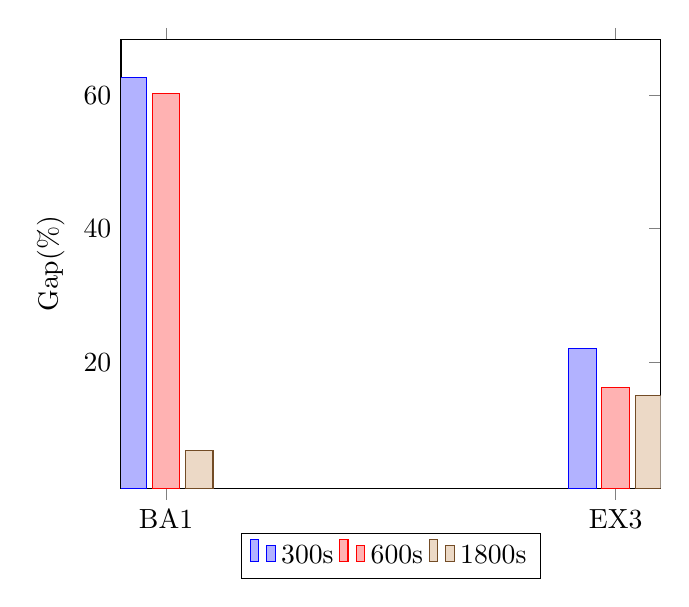
\begin{tikzpicture}
	\begin{axis}[
		ylabel=Gap(\%),
		symbolic x coords={BA1,EX3},
		xtick=data,
		legend style={at={(0.5,-0.1)}, anchor=north, legend columns=-1},
		ybar,
		]
		\addplot coordinates {(BA1, 62.7) (EX3, 22.0)};
		\addplot coordinates {(BA1, 60.3) (EX3, 16.2)};
		\addplot coordinates {(BA1, 6.76) (EX3, 15.0)};
		\legend{300s,600s,1800s}
	\end{axis}
\end{tikzpicture}\\
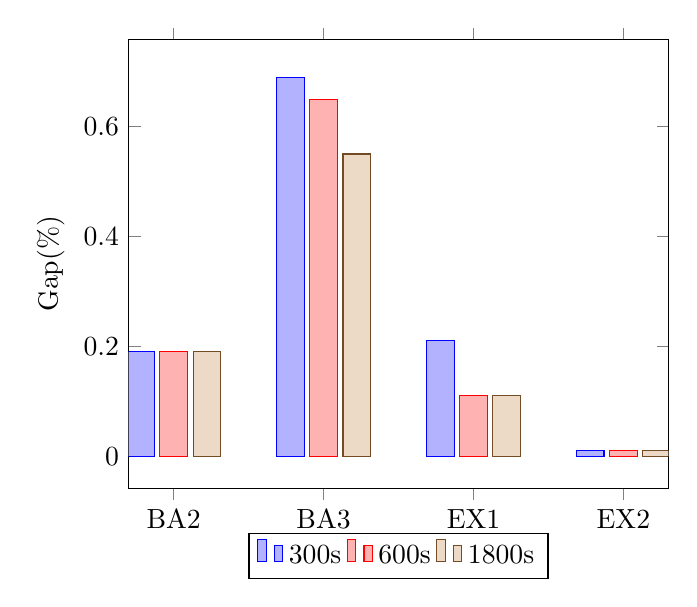
\begin{tikzpicture}
	\begin{axis}[
		ylabel=Gap(\%),
		symbolic x coords={BA2,BA3,EX1,EX2},
		xtick=data,
		legend style={at={(0.5,-0.1)}, anchor=north, legend columns=-1},
		ybar,
		]
		\addplot coordinates {(BA2, 0.19) (BA3, 0.69) (EX1, 0.21) (EX2, 0.01)};
		\addplot coordinates {(BA2, 0.19) (BA3, 0.65) (EX1, 0.11) (EX2, 0.01)};
		\addplot coordinates {(BA2, 0.19) (BA3, 0.55) (EX1, 0.11) (EX2, 0.01)};
		\legend{300s,600s,1800s}
	\end{axis}
\end{tikzpicture}
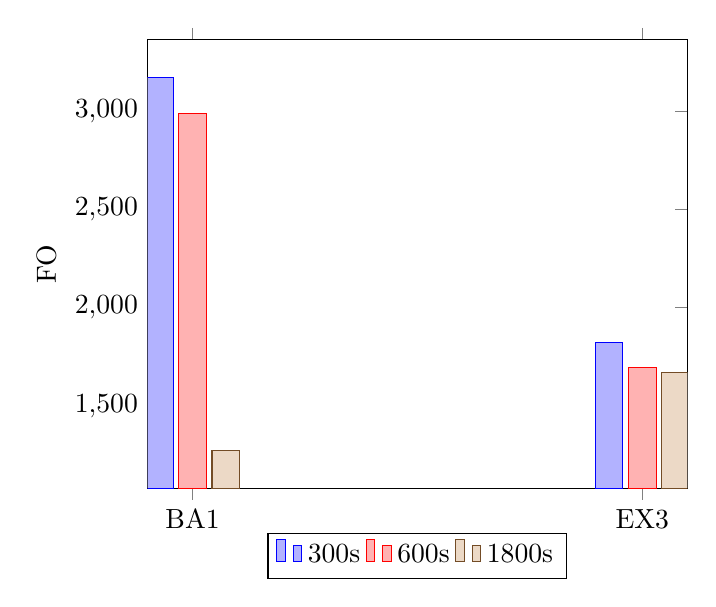
\begin{tikzpicture}
	\begin{axis}[
		ylabel=FO,
		symbolic x coords={BA1,EX3},
		xtick=data,
		legend style={at={(0.5,-0.1)}, anchor=north, legend columns=-1},
		ybar,
		]
		\addplot coordinates {(BA1, 3171.5) (EX3, 1819.7)};
		\addplot coordinates {(BA1, 2985.0) (EX3, 1693.9)};
		\addplot coordinates {(BA1, 1271.5) (EX3, 1669.3)};
		\legend{300s,600s,1800s}
	\end{axis}
\end{tikzpicture}
\end{center}
Questi risultati sono stati ottenuti eseguendo l'istanza una singola volta con il limite di tempo dato. Non sono stati impostati dei vincoli relativi a numero di thread o valori per il seed. Per quasi tutte le soluzioni, Gurobi segna uno stato per la soluzione pari a TIME\_LIMIT, in quanto, per via della natura del problema, trovare la soluzione ottima risulta complesso. Lo stato viene segnato come OPTIMAL per le soluzioni delle istanze EX1 e EX2 con un limite di tempo di 30 minuti. Sia per EX1 che per EX2, si nota però che Gurobi ha trovato una soluzione identica anche con altri limiti di tempo. Per l'istanza EX2 con tempo limite pari a 10 minuti, si nota che l'ultimo best bound trovato è di 10254.1 e non 10271.0 come riportato nella tabella: il best bound viene ottenuto mediante rilassamento e viene migliorato nel tempo grazie a varie tecniche, come cutting planes (es. Gomory), branch and bound, pruning o presolve. I valori ottimi inseriti nelle varie tabelle rappresentano il best bound trovato nei test sulle istanze con limite di tempo pari a 30 minuti e il gap individuato per ogni soluzione è stato ricalcolato sulla base di questo: se si osservano i log, per esempio si può osservare come il gap per la soluzione trovata per EX2 con tempo limite pari a 10 minuti sia uguale allo 0.18\%, in quanto calcolato rispetto al best bound citato prima di 10254.1.

\section*{Possibili estensioni e conclusioni}
\addcontentsline{toc}{section}{Possibili estensioni e conclusioni}
Capitolo dedicato a possibili estensioni e conclusioni sui dati. Prima di questo bisogna introdurre i grafici, per le estensioni possibili idee sono:
\begin{itemize}
	\item Shift design
	\item Basi di dati
	\item Ampliare finestra temporale
	\item Euristiche
	\item Grafica
	\item Client-Server
\end{itemize}

\appendix

\section{Valori dei coefficienti degli obiettivi}
\begin{center}
	\begin{tabular}{ c|c }
		$\lambda_1$ & 20.0\\
		$\lambda_2$ & 1.0\\
		$\lambda_3$ & 1.0\\
		$\lambda_4$ & 1.0\\
		$\lambda_5$ & 1.0\\
		$\lambda_6$ & 1.0\\
		$\lambda_7$ & -0.5\\
		$\lambda_8$ & -1.0\\
		$\lambda_{9over}$ & 3.0\\
		$\lambda_{9under}$ & 0.5\\
	\end{tabular}
\end{center}

% mostra tutte le citazioni anche se non sono state citate esplicitamente
\nocite{*}


\printbibliography

\section*{Ringraziamenti}
Desidero innanzitutto ringraziare la relatrice di questa tesi, Renata Mansini, per l’attenzione e la disponibilità dimostrate durante la stesura.

Ringrazio poi i miei nonni e mia sorella Isabel per il supporto mostrato nel corso di questi ultimi anni.

Ringrazio inoltre le persone che ho incontrato e che mi hanno aiutato durante questo percorso: “Il maritozzo fan club”, “Il gruppo di Yousef”, “Gli amici di Pietro”, “Il gruppo di Uovo”, Marco, Andrea e il gruppo di lavoro.

Infine, un ringraziamento particolare va a Francesco Sarubbi e Francesco Cominelli, senza i quali questa tesi non sarebbe stata possibile.
\end{document}